\section{Hindley-Milner Type Inference}

\subsection{Background on the Hindley-Milner Type System}
The Hindley-Milner Type System is a classical type system for the lambda calculus with parametric polymorphism (Wikipedia). Parametric polymorphism here refers to a way of making a language more expressive while maintaining full static type safety. More specifically, this means that we can write function or data types generically, like we may using generics in Java, and handle such values identically. This allows much more versatility in terms of types supported to achieve a certain outcome.

There are 2 well known algorithms within the domain of the Hindley-Milner Type System - Algorithm J and Algorithm W. In this project we will be focusing on Algorithm W, which is more generally considered to be \textit{the} HM algorithm. Algorithm J differs from Algorithm W in that substitutions are composed but applied only when essential, and it returns only the type assigned to a specific term instead of the whole type assignment. It can be seen as a precise application of Algorithm W. As students looking to implement a system with close relation to the fundamental formalism, we chose Algorithm W.

\subsection{The Expr Language}
    \begin{itemize}
        \item The expr language below defines the types of expressions in the HM Type System.
        \item Any extensions as coded in the implementation (such as binaryOp) are syntactic sugar for the following exprs.
    \end{itemize}
    \begin{alignat*}{3}
    expr &::= x &\\
     &| \quad \textit{expr expr} 
     &[application]\\
     &| \quad \text{fun $x \rightarrow$ } expr &[abstraction]\\
     &| \quad \text{let $x$ = } expr \text{ in } expr &[let]\\
     &| \quad \text{let $x$ = } expr &[globalLet]
    \end{alignat*}

Where $x$ is any valid identifier.
  
  
\subsection{Types}
The HM Type System consists of exprs that relate to two types.
  \begin{itemize}
    \item Monomorphic Types $\tau$.
    \item Polymorphic Types $\sigma$ (Type Schemes).
  \end{itemize}
  
  \begin{alignat*}{3}
\tau &::= \alpha & [typeVars]\\
 &| \quad \iota & [literals]\\
 &| \quad \tau \rightarrow \tau \quad & [funTypes]
\end{alignat*}
\begin{align*}
\iota &= \{\textit{int, string, bool}\}
\end{align*} 
\begin{align*}
\sigma &::= \tau \\
 &| \quad \forall \alpha \hspace{2} \sigma
\end{align*}

Where $\alpha$ refers to any variable. Monomorphic means that every value has a single, unique type, while polymorphic means that values may have more than one type.

\subsection{Instantiation}
  \begin{itemize}
    \item Instantiation refers to the substitution of a polymorphic Type Scheme that results in a monomorphic type. Example:
    \end{itemize}
    
    \begin{center}
Let $\sigma = \forall\alpha_1. \alpha_1 \rightarrow\alpha_1$, \\
and $S = \{\alpha_1 \mapsto string\}$ \\
then $S\sigma = string \rightarrow string$
 \end{center}
 
    \begin{itemize}
    \item Generic Instantiation refers to the substitution of a polymorphic Type Scheme that results in another polymorphic Type Scheme.
    \item To discuss Generic Instantiation, we need to introduce the partial order $\sqsubseteq$ defined as a way to relate the generality of different Type Schemes.
  \end{itemize}
  \begin{alignat*}{1}
&\frac{\tau' = \{\alpha_i\mapsto\tau_i\}\tau \quad \beta_i\notin free(\forall \alpha_1...\alpha_n.\tau)}{\forall\alpha_1...\alpha_n.\tau \sqsubseteq \forall\beta_1...\beta_m.\tau'} [Specialisation]
\end{alignat*} 

\begin{itemize}
    \item An example of Generic Instantiation:
  \end{itemize}
  
  \begin{center}
      Let $\sigma = \forall\alpha_1. \alpha_1\rightarrow\alpha_1$, \\
and $S = \{\alpha_1 \mapsto (int \rightarrow\beta_1)\}$ \\
then $S\sigma = \forall \beta_1. (int \rightarrow\beta_1) \rightarrow (int \rightarrow\beta_1)$
  \end{center}
  
\subsection{Unification}
  \begin{itemize}
    \item Unification is the process of finding the Most General Unifier (MGU) which is a substitution that makes two terms look identical.
    \item Unification (figure \ref{fig:unification}) is a necessary part of the HM Type System as it is used to ensure inferred types are consistent, and as it allows the system to gain more information about types.
  \end{itemize}
  
  \begin{figure}[H]
      \centering
      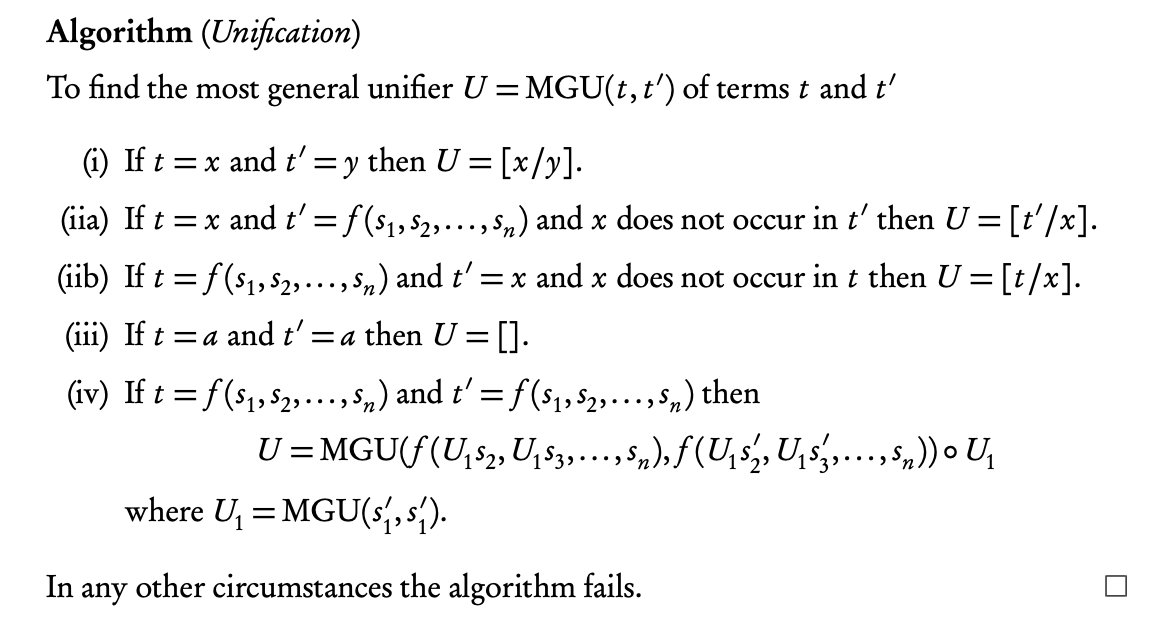
\includegraphics[width=0.8\linewidth]{images/unification.png}
      \caption{Pseudocode unification algorithm by Ian Grant}
      \label{fig:unification}
  \end{figure}

\subsection{Inference Rules}
  \begin{itemize}
    \item To discuss the syntactic inference rules of a HM Type System, we introduce the notion of a context (or set of assumptions) $\Gamma$.
    \item With $\Gamma$, we can make inferences using the $\vdash$ operator.
  \end{itemize}
  \begin{alignat*}{2}
\Gamma &::= \epsilon\\
 &| \quad \Gamma, x:\sigma
\end{alignat*}
\begin{alignat*}{2}
\Gamma \vdash expr&:\sigma
\end{alignat*}
\begin{itemize}
\item We now have all the information to define our rules of inference.
  \end{itemize}
  \begin{alignat*}{1}
&\frac{x:\sigma \in \Gamma \quad \sigma\sqsubseteq\tau}{\Gamma \vdash x:\tau} [Var] \\ \\
&\frac{\Gamma \vdash e_0: \tau\rightarrow\tau' \quad \Gamma \vdash e_1:\tau}{\Gamma \vdash e_0 e_1:\tau'} [App] 
\end{alignat*}
\begin{alignat*}{1}
&\frac{\Gamma, x:\tau \vdash e:\tau'}{\Gamma \vdash \text{fun $x \rightarrow$ } e:\tau\rightarrow\tau'} [Abs] \\ \\
&\frac{\Gamma \vdash e_0: \tau \quad \Gamma, x:\bar\Gamma(\tau) \vdash e_1:\tau'}{\Gamma \vdash \text{let $x$ = } e_0 \text{ in } e_1:\tau'} [Let]
\end{alignat*}
\begin{center}
    $\bar\Gamma(\tau) = \forall \hat\alpha.\tau \quad \quad \hat\alpha=free(\tau) - free(\Gamma)$
\end{center}
  
\subsection{Implementation}
The main logic of our implementation for the HM Type System relates directly to each of the rules of inference.
  \begin{itemize}
    \item For the [Var] rule:
  \end{itemize}
  \begin{figure}[H]
      \centering
      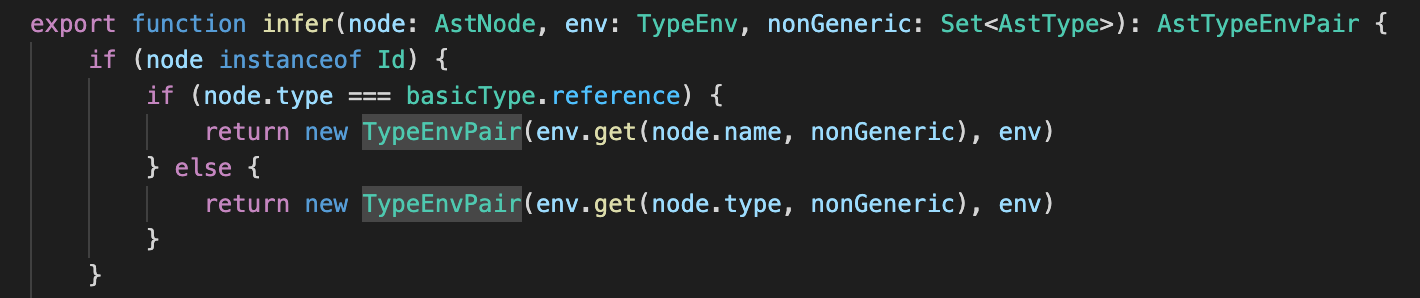
\includegraphics[width=0.8\linewidth]{images/var.png}
      \caption{Implementation of var rule}
      \label{fig:varrule}
  \end{figure}
  \begin{itemize}
    \item For the [App] rule:
  \end{itemize}
  \begin{figure}[H]
      \centering
      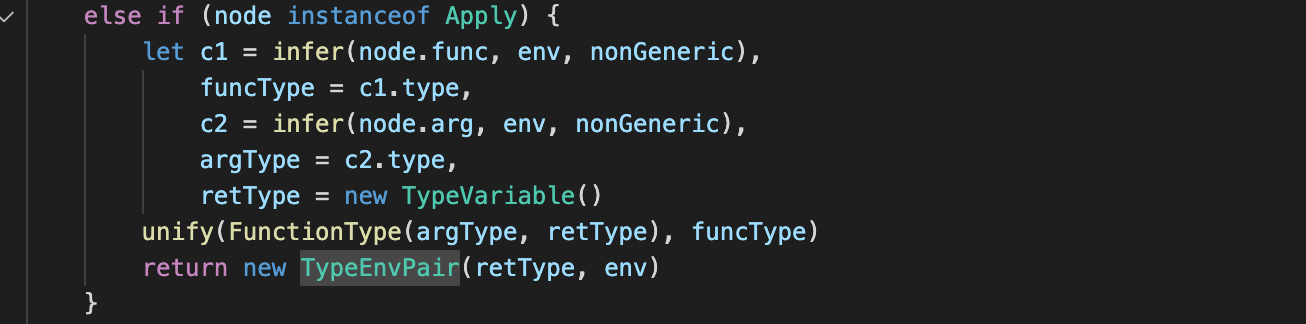
\includegraphics[width=0.8\linewidth]{images/app.png}
      \caption{Implementation of app rule}
      \label{fig:apprule}
  \end{figure}
  \begin{itemize}
    \item For the [Abs] rule:
  \end{itemize}
  \begin{figure}[H]
      \centering
      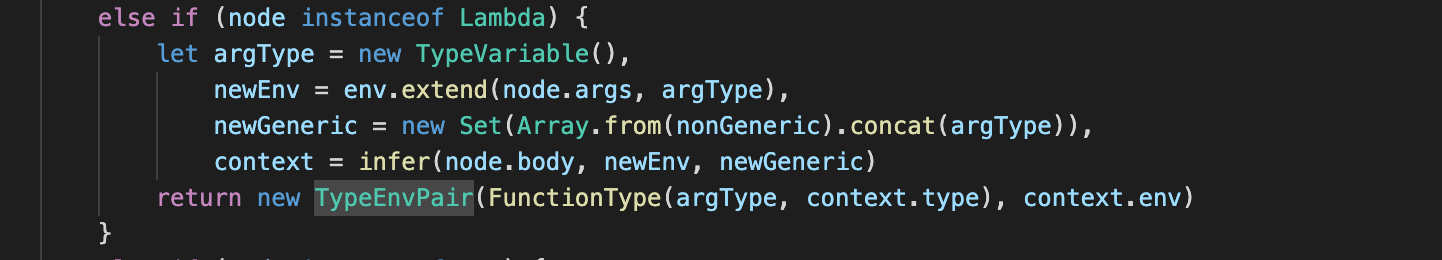
\includegraphics[width=0.8\linewidth]{images/abs.png}
      \caption{Implementation of abs rule}
      \label{fig:absrule}
  \end{figure}
  \begin{itemize}
    \item For the [Let] rule:
  \end{itemize}
  \begin{figure}[H]
      \centering
      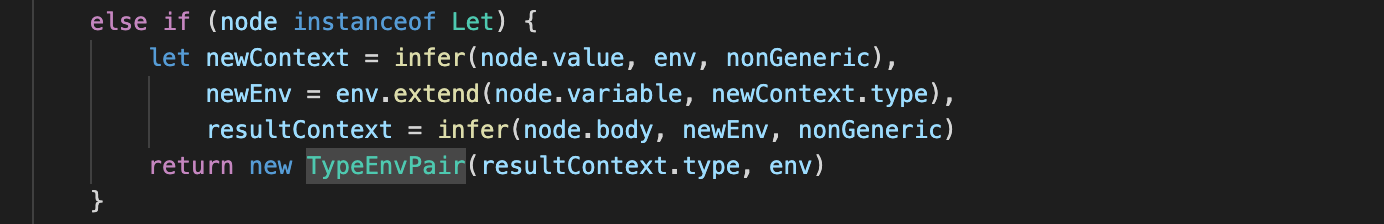
\includegraphics[width=0.8\linewidth]{images/let.png}
      \caption{Implementation of let rule}
      \label{fig:letrule}
  \end{figure}
  \begin{itemize}
    \item The following [GlobalLet] rule is an extension of the original HM Type System. To introduce the persistence required by a global let rule, we need to ensure that the environment persists. Therefore, all our rules return a \verb#TypeEnvPair# object for this purpose.
    \item For the [GlobalLet] rule:
  \end{itemize}
  \begin{figure}[H]
      \centering
      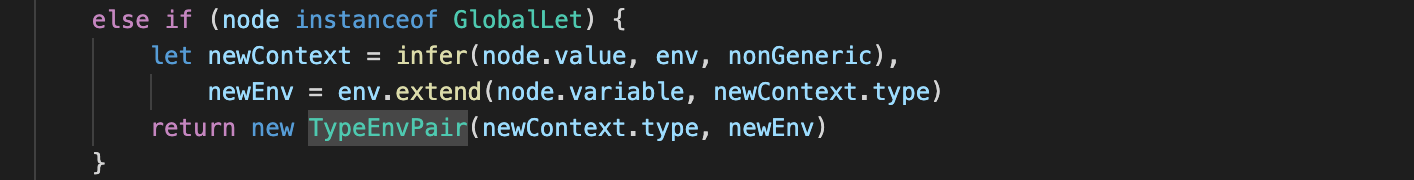
\includegraphics[width=0.8\linewidth]{images/globalLet.png}
      \caption{Implementation of globalLet rule}
      \label{fig:globalLetrule}
  \end{figure}
  \begin{itemize}
    \item As an example of extending the HM Type System to additional syntax, we add an example below of the BinaryOp rule, which can be decomposed to the rules above.
    \item For the [BinaryOp] rule:
  \end{itemize}
  \begin{figure}[H]
      \centering
      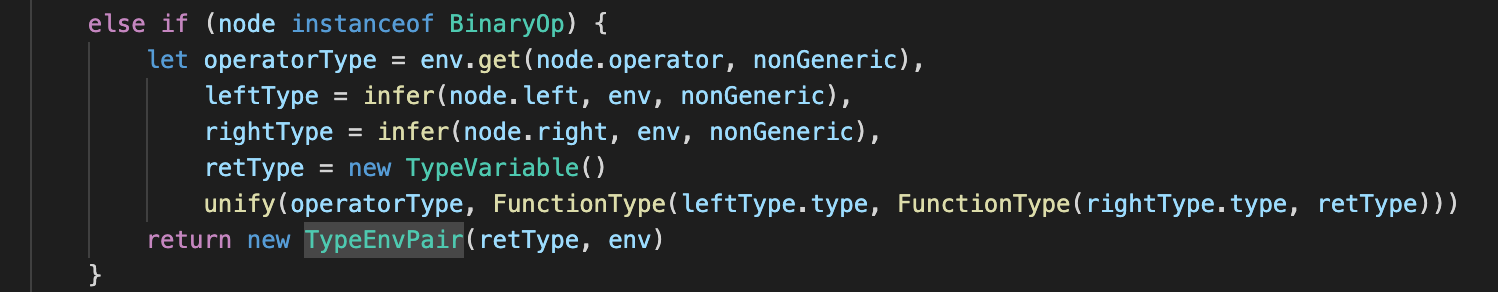
\includegraphics[width=0.8\linewidth]{images/binaryOp.png}
      \caption{Implementation of binaryOp rule}
      \label{fig:binaryOprule}
  \end{figure}
  
\subsection{Exponential Case}
Algorithm W has an exponential case that we feel is worth discussing. In certain cases like deeply-nested let bindings, the size of the type inferred increases exponentially. Here is an example to demonstrate this, where we make use of \verb|let|, function definition, and the method pair that we have implemented:

\footnotesize
\begin{verbatim}
let dup = fun x -> (pair x x);;
Inferred type of size 2^0: 
(t0 -> (t0 * t0))

let dup2 = dup dup;;
Inferred type of size 2^1: 
((t1 -> (t1 * t1)) * (t1 -> (t1 * t1)))

let dup3 = dup dup2;;
Inferred type of size 2^2: 
(((t2 -> (t2 * t2)) * (t2 -> (t2 * t2))) * ((t2 -> (t2 * t2)) * (t2 -> (t2 * t2))))
\end{verbatim}
\normalsize

As observed, the size of the type inferred increases exponentially. This can make the static type checking inefficient and resource intensive. In practice, however, this may be relatively uncommon. Thus, the type inference algorithm can be considered to enjoy polynomial time complexity \textit{in general}.
